\section{Efficient Sorting}

\subsection{Merge Algorithm}

		\defn{Sentinel}{a number which is much larger than any other number in the
		array. It can be represented by \texttt{Integer.MAX\_VALUE}}

		\rem{A more general definition sees sentinel as any value which is interpreted
		as a condition to terminate the algorithm}

		\defn{Stable}{an algorithm which preserves the input order of repeated elements}

		\rem{note that this is only relevant if the repeated elements are somehow
		distinguishable (e.g deck of cards , (rank,value))}

		\defn{Key}{for data being recorded as a tuple of values, the key is the value
		used to sort (e.g (name, surname) , K=S)}

		\defn{Merging Algorithm}{an algorithm which takes two sorted sequences and
		returns a single combined sequence~\cite{merge}}

\subsubsection{Overview}

		\par{The merge algorithm takes an unsorted array and 3 indices, it then splits
		the array into two subarrays and copies each subarray into memory. Finally, it
		iterates over every element of the original array, for each iteration it
		compares the current elements of the 2 subarrays against each other, replacing
		the appropriate value into the original array and increasing the index of the
		subarray by $1$}

\subsubsection{Formal Definition}

\begin{algorithm}[H]
	\DontPrintSemicolon
	\SetAlgoLined\KwData{Array $A$ , indeces $p,q,r$}
	\SetKwFunction{KwFn}{Merge}
	\KwResult{sorted subarray $A[p..r]$}
	\KwFn{A,p,q,r}\\
	$n_1$ := q - p + 1{\tcc*[r]{initialize subarrays' size}}\;
	$n_2$ := r - q\;
	L[0..$n_1$] := A[p..q]{\tcc*[r]{copy to subarrays}}\;
	R[$n_2$..r] := A[q+1..r]\;
	L[$n_1$] := $\infty${\tcc*[r]{add the sentinel values to end of
subarrays}}\;
	R[$n_2$] := $\infty$\;
	i,j := 0\;
	\For{k=p \KwTo r}{\;
	    \uIf{L[i] $\leq$ R[j]}{\;
			A[k] := L[i]\;
			i := i + 1\;
		}
		\uElse{\;
			A[k] := R[j]\;
			j := j + 1\;
		}
	}
		\caption{Merge}
\end{algorithm}

\subsubsection{Properties}

		\begin{itemize}
			\item\textbf{Running Time : } $O(n)$ , since the initialization of
the $L , R$ subarrays takes $O(n)$ and the loop is executed $n$ times and
contains only constant-time operations
			\item\textbf{Stable}
			\item\textbf{Memory Requirements : } $O(n)$ to store $L, R$	
		\end{itemize}

\subsection{Merge-Sort}

\rem{See informal definition in previous section}

\subsubsection{Formal Definition}

	\begin{algorithm}[H]
	\DontPrintSemicolon
	\SetAlgoLined\KwData{Array $A$ , indeces $p,r$}
	\SetKwFunction{KwFn}{Merge-Sort}
	\SetKwFunction{KwFn2}{Merge}
	\KwResult{sorted array $A[p..r]$}
	\KwFn{A,p,r}\\
	\uIf{p < r}{
		q := (p + r) / 2\;
		\KwFn(A,p,q)\;
		\KwFn{A,q+1,r}\;
		\KwFn2{A,p,q,r}\;
	}
	\caption{Merge-Sort Algorithm}
	\end{algorithm}

\subsubsection{Execution \& Properties}

\rem{to sort an array $A$ with $n$ elements, we would call
\texttt{MERGE-SORT(A,0,n-1)}}

\par{Note how the algorithm gives rise to a binary recursive tree, since we
split each subarray into 2 with each iteration until we hit the stopping
condition (single element array). So, the first subarray is entirely sorted,
before the second \texttt{MERGE-SORT} call. The two \ita{half-subarrays} returned
from each call are then merged by calling \texttt{MERGE}. The process is then
repeated in the right branch}

\begin{figure}[H]
	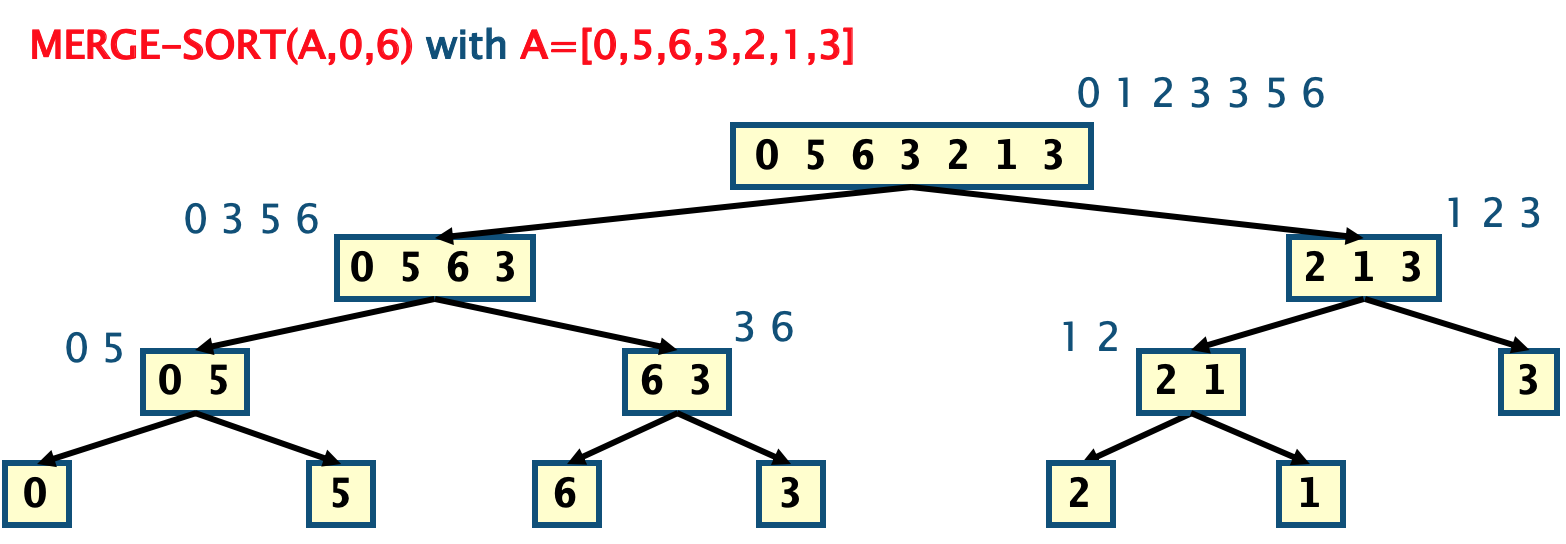
\includegraphics[width=\textwidth]{mergeTree}
\end{figure}

\begin{itemize}
	\item\textbf{Stable}
	\item\textbf{Memory} $O(n)$
	\item\textbf{Running Time} $O(n \log n)$
\end{itemize}

\subsection{Recurrence Equations}


\defn{Recurrence Equation}{describe the overall running time of a problem of
size $n$ in terms of the running time on smaller inputs}
	

\par{Recursive algorithms can be described via \ita{recurrence equations}. Take
$t(n)$ to denote the \ita{worst-case} running time of \texttt{MERGE-SORT(n)},
then we can characterize $t(n)$ by means of an equation where $t(n)$ is
recursively expressed in terms of itself.
}
\par{If \texttt{MERGE-SORT(n)} has running time $T(n)$ then, each recursive call
will \texttt{MERGE-SORT(n/2)} will run on $T(n/2)$ time. Hence, we can define
$T(n)$ recursively as follows}

$$ T(n) = \left\{ 
	\begin{array}{ll}
		b & n \leq 1 \quad \text{(base case)} \\
		2T(n/2) + cn 
	\end{array}
\right.
$$
\subsubsection{Iterative Method}
\par{Though correct, a more informative definition will be one that does not
involve $T(n)$ itself. From its \ita{closed-form} characterization, we can
define it in \ita{big-Oh} terms. We do this, by iterative substitution on the
RHS of the recurrence relation until the base case is reached}
\par{Continuing with the expression above, if we substitute $n$ by $n/2$ in the RHS we
essentially double the children arrays, and we get}

\begin{align*}
	T(n) &= 2(2T((n/2)/2) + c(n/2)) + cn \\
		&= 2^2t(n/2^2) + 2(cn/2) + cn \\
		&= 2^2t(n/2^2) + 2cn
\end{align*}

\par{If we repeat the process, assuming that $n$ is relatively large, then we
find the general pattern}

$$t(n) = 2^it(n/2^i) +  icn$$

\par{In order to determine the base case, we look at the original definition,
and observe that  we need to find $t(n)$ , for $n \leq 1$. Given our general
argument $\frac{n}{2^i}$ we need $2^i = n \iff i = \log n$. Hence, substituting
$i$ by $ \log n$ gives}

\begin{align*}
	t(n) &= 2^{\log n} t(n/2^{\log n}) + cn\log n \\
		&= nt(1) + cn\log n \\
		&= nb + cn\log n
\end{align*}

\par{Lastly, since $b,c$ are constants, we have shown that $t(n)$ is $O(n\log
n)$}

\subsubsection{Master Method}

	\par{There is a general form of recurrence relation that arises in the
analysis of the divide-and-conquer algorithms}

$$T(n) = aT(n/b) + f(n) \qquad a , b \geq 1$$

	\par{Then, for $f(n) = \Theta(n^c)$ , the solution will be one of the
following 3 cases}

	\begin{enumerate}
		\item $
\mathrm{c}<\log _{\mathrm{b}} \mathrm{a} \text { then } \mathrm{T}(\mathrm{n})=\Theta\left(n^{\log _{b} a}\right)
$
		\item $
\mathrm{c}=\log _{\mathrm{b}} \mathrm{a} \text { then } \mathrm{T}(\mathrm{n})=\Theta(\mathrm{n} \leq \log \mathrm{n})
$
		\item $
\mathrm{c}>\log _{\mathrm{b} 2} \mathrm{a} \text { then } \mathrm{T}(\mathrm{n})=\Theta(\mathrm{f}(\mathrm{n}))
$
	\end{enumerate}

\par{For \texttt{MERGE-SORT}, we have $a=2 , b=2 , f(n) = \Theta(n) , c = 1$ .
Hence, the solution is given by case $2$ , $\Theta(n^c \log n) = \Theta(n \log
n)$}

\subsubsection{Tree Method}

\rem{See lecture 5 slides 52-60}


\subsection{Quicksort}

